% v2-acmsmall-sample.tex, dated March 6 2012
% This is a sample file for ACM small trim journals
%
% Compilation using 'acmsmall.cls' - version 1.3 (March 2012), Aptara Inc.
% (c) 2010 Association for Computing Machinery (ACM)
%
% Questions/Suggestions/Feedback should be addressed to => "acmtexsupport@aptaracorp.com".
% Users can also go through the FAQs available on the journal's submission webpage.
%
% Steps to compile: latex, bibtex, latex latex
%
% For tracking purposes => this is v1.3 - March 2012

\documentclass[prodmode,acmtecs]{acmsmall} % Aptara syntax

\usepackage{caption}
\usepackage{subfig}

% Metadata Information
% \acmVolume{9}
% \acmNumber{4}
% \acmArticle{39}
% \acmYear{2010}
% \acmMonth{3}

% Copyright
%\setcopyright{acmcopyright}
%\setcopyright{acmlicensed}
%\setcopyright{rightsretained}
%\setcopyright{usgov}
%\setcopyright{usgovmixed}
%\setcopyright{cagov}
%\setcopyright{cagovmixed}
%
% % DOI
% \doi{0000001.0000001}
%
% %ISSN
% \issn{1234-56789}

% Document starts
\begin{document}

% Page heads
\markboth{B. Berger et al.}{Title}

% Title portion
\title{Title}
\author{BONNIE BERGER
\affil{Massachusetts Institute of Technology}
NOAH M. DANIELS
\affil{Massachusetts Institute of Technology}
Y. WILLIAM YU
\affil{Massachusetts Institute of Technology}}


\begin{abstract}
abstract goes here
\end{abstract}


%
% The code below should be generated by the tool at
% http://dl.acm.org/ccs.cfm
% Please copy and paste the code instead of the example below. 
%
% \begin{CCSXML}
% <ccs2012>
%  <concept>
%   <concept_id>10010520.10010553.10010562</concept_id>
%   <concept_desc>Computer systems organization~Embedded systems</concept_desc>
%   <concept_significance>500</concept_significance>
%  </concept>
%  <concept>
%   <concept_id>10010520.10010575.10010755</concept_id>
%   <concept_desc>Computer systems organization~Redundancy</concept_desc>
%   <concept_significance>300</concept_significance>
%  </concept>
%  <concept>
%   <concept_id>10010520.10010553.10010554</concept_id>
%   <concept_desc>Computer systems organization~Robotics</concept_desc>
%   <concept_significance>100</concept_significance>
%  </concept>
%  <concept>
%   <concept_id>10003033.10003083.10003095</concept_id>
%   <concept_desc>Networks~Network reliability</concept_desc>
%   <concept_significance>100</concept_significance>
%  </concept>
% </ccs2012>
% \end{CCSXML}
%
% \ccsdesc[500]{Computer systems organization~Embedded systems}
% \ccsdesc[300]{Computer systems organization~Redundancy}
% \ccsdesc{Computer systems organization~Robotics}
% \ccsdesc[100]{Networks~Network reliability}

%
% End generated code
%

% We no longer use \terms command
%\terms{Design, Algorithms, Performance}

\keywords{computational biology, database search, metagenomics, chemogenomics}

\acmformat{Bonnie Berger, Noah M. Daniels,
and Y. William Yu, 2015. Title.}
% At a minimum you need to supply the author names, year and a title.
% IMPORTANT:
% Full first names whenever they are known, surname last, followed by a period.
% In the case of two authors, 'and' is placed between them.
% In the case of three or more authors, the serial comma is used, that is, all author names
% except the last one but including the penultimate author's name are followed by a comma,
% and then 'and' is placed before the final author's name.
% If only first and middle initials are known, then each initial
% is followed by a period and they are separated by a space.
% The remaining information (journal title, volume, article number, date, etc.) is 'auto-generated'.

\begin{bottomstuff}
% This work is supported by the National Science Foundation, under
% grant CNS-0435060, grant CCR-0325197 and grant EN-CS-0329609.
%
% Author's addresses: G. Zhou, Computer Science Department,
% College of William and Mary; Y. Wu  {and} J. A. Stankovic,
% Computer Science Department, University of Virginia; T. Yan,
% Eaton Innovation Center; T. He, Computer Science Department,
% University of Minnesota; C. Huang, Google; T. F. Abdelzaher,
% (Current address) NASA Ames Research Center, Moffett Field, California 94035.
\end{bottomstuff}

\maketitle


\section{Introduction}

Computational biologists answer biological and biomedical 
questions by using computation in support of---or in place of---laboratory 
procedures, in hopes of obtaining more accurate answers at a greatly reduced 
cost.
The past two decades have seen unprecedented technological progress with regard
to generating biological data; next-generation sequencing, mass spectroscopy,
microarrays, nuclear magnetic resonance, and other high-throughput approaches
have led to an explosion of data.
This explosion of data is a mixed blessing.
On the one hand, the scale and scope of data should allow new insights into
genetic and infections diseases, cancer, basic biology, and even human migration
patterns.
On the other hand, researchers are generating datasets so massive that it has 
become difficult to analyze them to discover patterns that give clues to the 
underlying biological processes.

Certainly, computers are getting faster and more economical; the amount of 
processing available per dollar of compute hardware is more or less doubling 
every year or two; a similar claim can be made about storage capacity 
(Figure~\ref{fig:growth}).
In 2002, when the first human genome was sequenced, the growth in computing 
power was still matching the growth rate of genomic data.
However, the sequencing technology used for the Human Genome Project--Sanger
sequencing--was supplanted around 2004, with the advent of what is now known as 
next-generation sequencing.
The material costs to sequence a genome have plummeted in the past
decade, to the point where a whole human genome can be sequenced for less than
one thousand U.S. Dollars.
As a result, by some estimates, the amount of genomic data available to 
researchers is increasing by a factor of 10 every year.

\begin{figure}[htb!]
\centering
\subfloat[Growth of genomic sequence data as compared with the combined power of the top-500 supercomputer list; y-axis is logarithmic]{
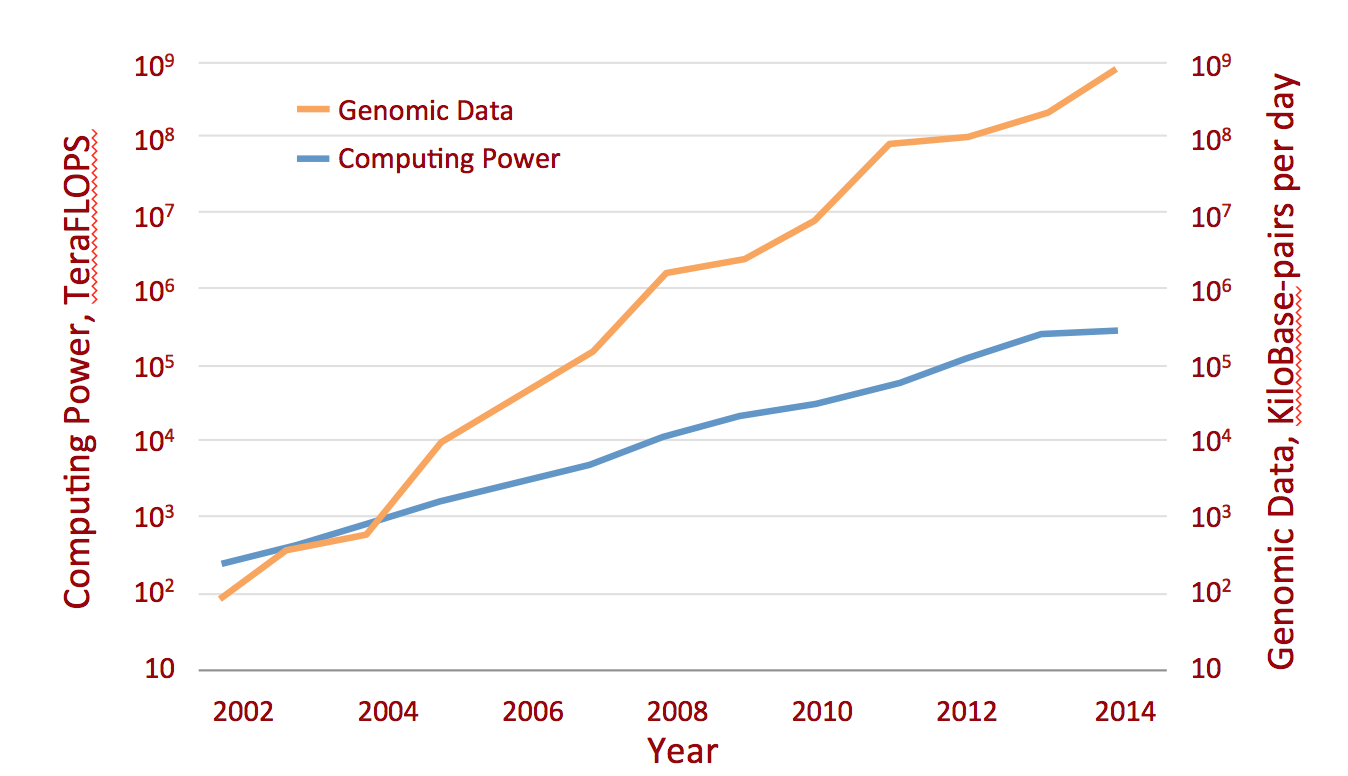
\includegraphics[width=3.0in]{assets/moore.png}
\label{fig:moore}
}\\
\subfloat[Growth of genomic sequence data as compared with hard drive capacity; y-axis is logarithmic]{
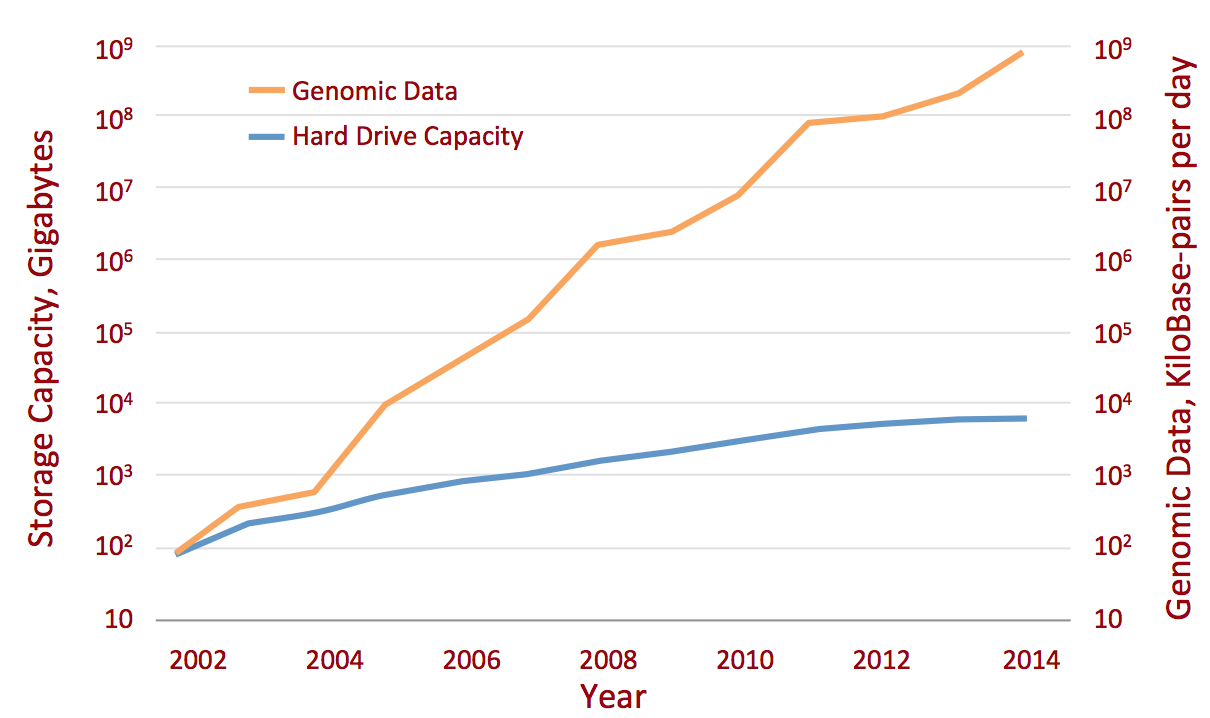
\includegraphics[width=3.0in]{assets/kryder.png}
\label{fig:kryder}
}
\caption[Sequencing vs. Storage]{Moore's and Kryder's laws contrasted with genomic sequence data}
\label{fig:growth}
\end{figure}

This growth in data poses significant challenges for 
researchers~\cite{marx2013biology}.
Currently, many omics applications require us to store, access, and analyze
large libraries of data.
One approach to solving these challenges is to embrace cloud computing.
Google, Inc. and the Broad Institute have teamed up to bring the GATK (Genome 
Analysis Toolkit) to the Google cloud (https://cloud.google.com/genomics/gatk).
ALSO MENTION AMAZON AWS HERE.
However, while cloud computing frees researchers from maintaining their own
data centers, and provides cost-saving benefits when computing resources are
not needed around the clock, it is no panacea.
First, in the face of disease outbreaks such as the 2014 Ebola virus epidemic 
in West Africa, analysis resources are needed at often-remote field sites.
While it is now possible to bring sequencing equipment and limited computing 
resources to remote sites, internet connectivity is still highly constrained.
Thus, accessing cloud resources for analytics may not be possible.
Moreover, cloud computing does not truly address the problem posed by
a corpus of data that is growing faster than Moore's law, because the computer
systems that make up those cloud datacenters are still themselves bound by
improvements in semiconductor technology; they still follow the trajectory
suggested by Moore's law.

ALGORITHMS FOR COMING UP WITH NOVEL BIOLOGICAL INSIGHTS not FOCUS OF THIS REVIEW
STORAGE REQUIREMENTS, NETWORK TRANSMISSION, ETC.

Computer scientists routinely exploit peculiarities in the structure of data in
order to reduce time or space complexity.
In computational biology, this approach has served researchers well.
Now-classical approaches such as principal component analysis (PCA) reduce the 
dimensionality of data in order to simplify analysis and uncover salient 
features.

\section{Biological sequence data and next-generation sequencing}

Many, but not all, of the problems in computational biology deal with sequence
data, either nucleotide sequences (nominally a four-letter alphabet) or protein
sequences (nominally a twenty-letter alphabet).
Certainly, as sequencing is generating the greatest volume of biological data,
a large portion of bioinformatics algorithms deal primarily with string data.
For the problem of exact search, approaches for transforming and indexing 
string data provide benefits.
The Burrows-Wheeler transform (BWT)~\cite{burrows1994block} provides efficient string 
compression through a reversible transformation, while the FM-index data 
structure~\cite{ferragina2000opportunistic} is a compressed substring index, based
on the BWT, which provides efficient storage as well as fast search.
Modern next-generation sequencing (NGS) technologies read short fragments of
DNA, known as \emph{reads}~\ref{fig:shotgun}, which must be mapped onto a reference sequence~\ref{fig:ngs-pipeline}
BWA (Burrows-Wheeler Aligner)~\cite{li2009fast} uses the BWT, while the 
Bowtie2~\cite{langmead2012fast} aligner further relies on the FM-index for efficient 
mapping of NGS reads.



\begin{figure}[htb!]
\centering
\subfloat[``Shotgun'' sequencing breaks DNA molecules into many short fragments, or reads, and relies on high coverage to produce a statistically likely representation of a whole genome]{
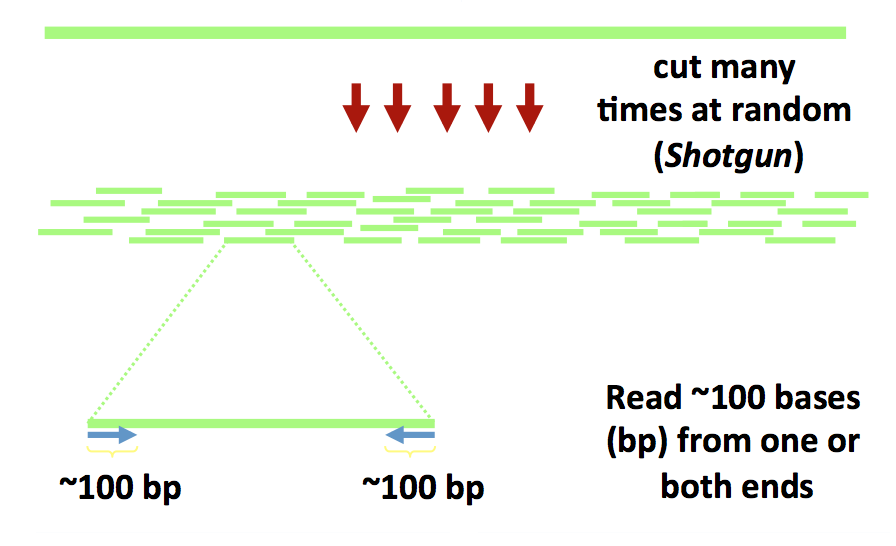
\includegraphics[width=3.0in]{assets/shotgun.png}
\label{fig:shotgun}
}
\subfloat[Single-nucleotide polymorphisms, or SNPs, are the simplest type of genomic variant, and form the bulk of ``variant-calling'' analysis]{
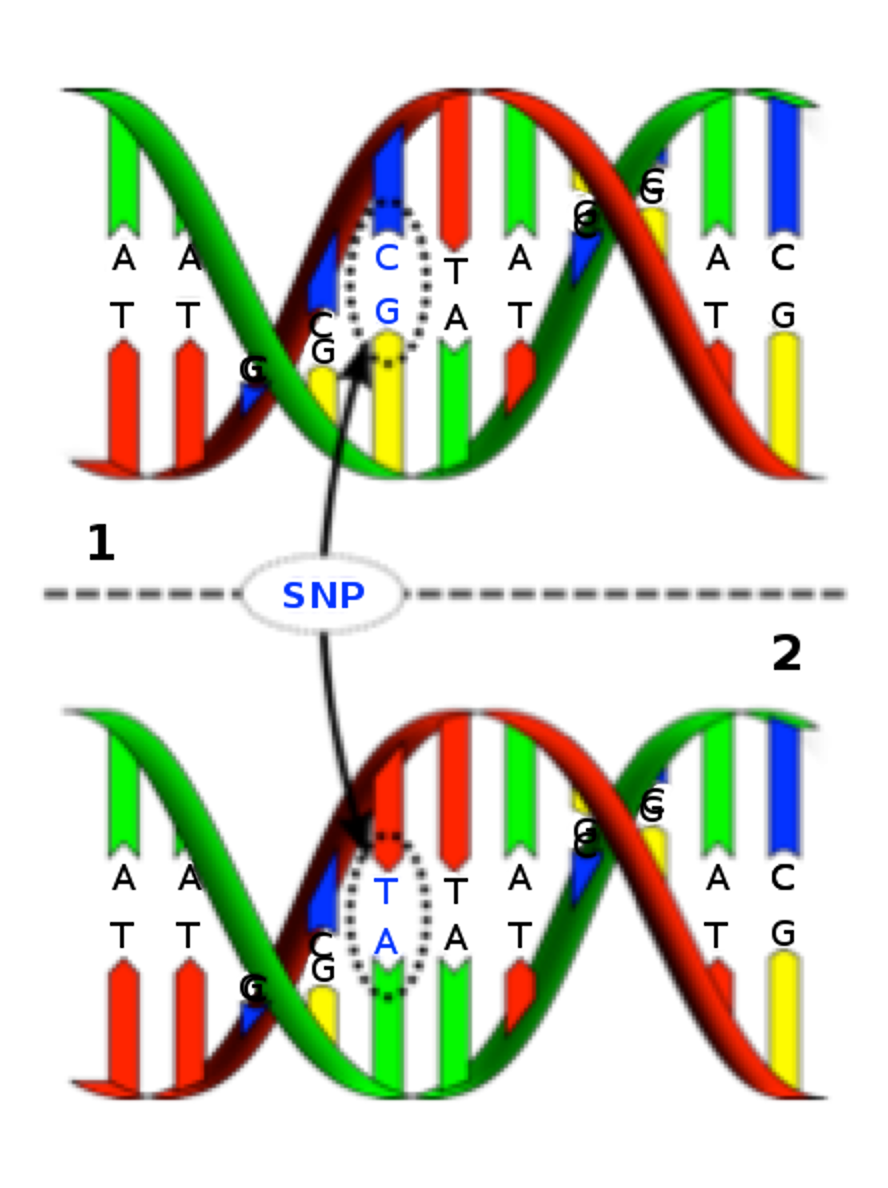
\includegraphics[width=3.0in]{assets/snps.png}
\label{fig:snps}
}\\
\subfloat[The NGS downstream analysis pipeline. Shotgun reads are mapped to a reference genome with tools such as BWA or Bowtie. The resulting genomic sequence is analyzed for variants with tools such as GATK or Samtools. This allows relationships between genes and diseases to be uncovered.]{
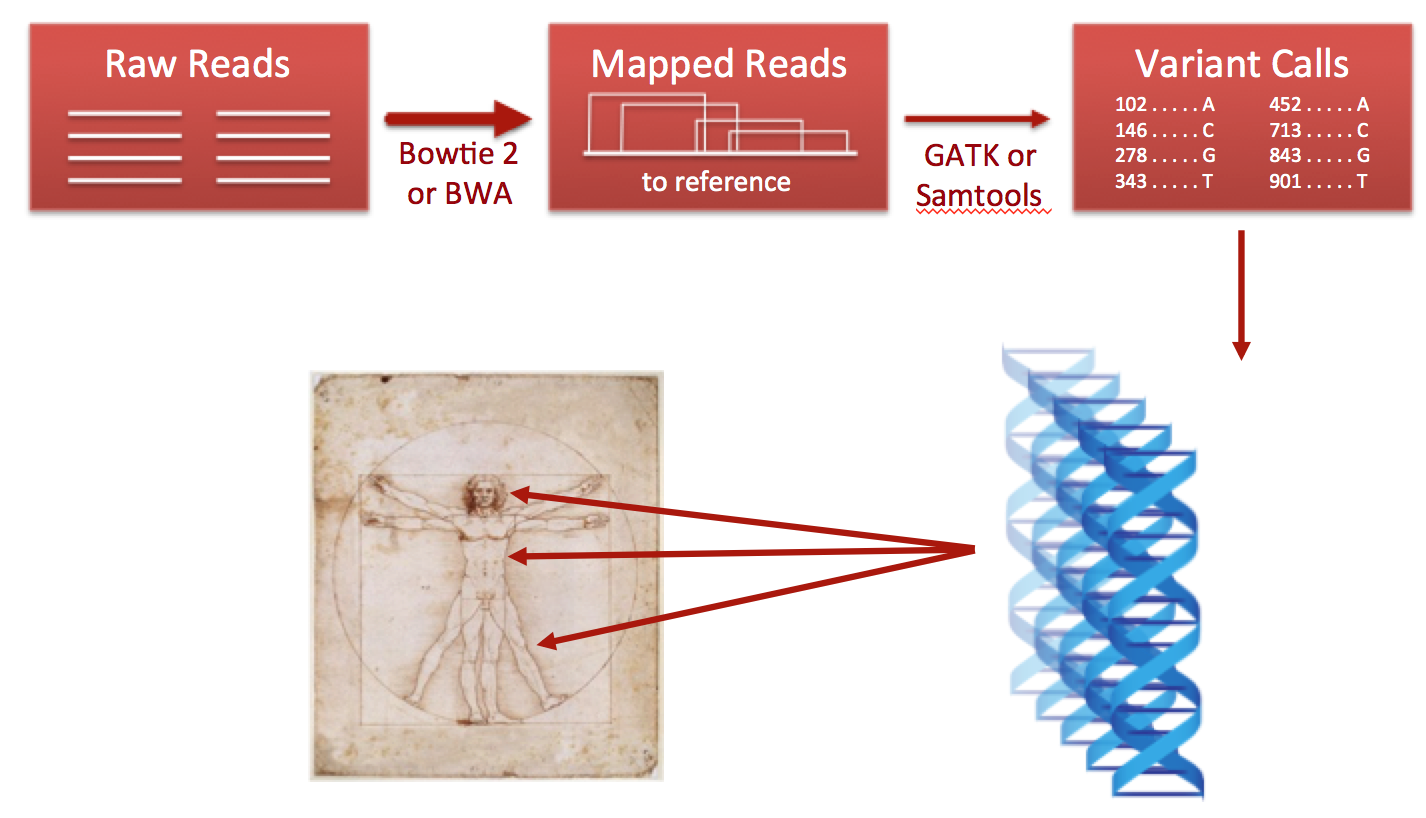
\includegraphics[width=3.0in]{assets/ngs-pipeline.png}
\label{fig:ngs-pipeline}
}
\caption[The NGS Pipeline]{The next-generation sequencing (NGS) pipeline.}
\label{fig:ngs}
\end{figure}

As biological sequence data is string data, it is frequently useful to index or
count instances of $k$-mers of a fixed length, $k$.
Search tools such as BLAST~\cite{altschul1990basic} rely on $k$-mer \emph{seeds} in a 
seed-and-extend approach to sequence search and alignment.
For counting $k$-mer frequencies, Jellyfish~\cite{marccais2011fast} relies on an efficient
hash-table encoding as well as Intel's ``compare-and-swap'' CPU instructions for
improved run-time performance.

Seeking to take advantage of sequence redundancy, \cite{loh2012compressive}
introduced \emph{compressive genomics}, an approach that relies on compressing
data in such a way that the desired computation (such as BLAST search) can be
performed in the compressed representation.
This approach 

(now, redundancy and compressive) loh2012compressive


Make use of a completely different paradigm for the structure of biological data. By combining redundancy with a low fractal dimension, able to develop algorithms that scale.

Next-gen sequencing, and some applications
Slide 27 to illustrate how sequencing works (2a, 2b)
Slide 28: sequence analysis pipeline (2c)
Redundancy - 
- 1000 genomes project, flybase, wormbase
- subsequence similarity (k-mer approaches)

Quality score compression

lossy compression - quartz

Mince~\cite{patro2015data} groups similar reads (those that share a common 
substring) together into ``buckets'', allowing that common substring to now be 
removed and treated as the bucket label, so that each read in the compressed 
representation comprises only its unique differences from the bucket label.
This allows a general-purpose compressor to achieve tight compression.

\section{Non-sequence data}

Another important type of biological data is gene expression, or the quantity of
a particular gene product (usually a protein) present in the cell.
Gene expression data is useful for relating genotype to phenotype, and is 
important in studying diseases including cancer.
Usually obtained through microarrays or RNA-seq technologies, expression data is
quantitative, as each gene from a sample is associated with a numeric expression
level, and high-dimensional, as many thousands of genes may be analyzed at a
time.
While expression data lends itself to cluster analysis and probabilistic 
approaches, the high dimensionality presents challenges.
Principal Component Analysis has shown promise in reducing the dimensionality
of gene expression data~\cite{raychaudhuri2000principal, alter2000singular, yeung2001principal, misra2002interactive}.
[NEED CITATIONS FOR DIFFICULTIES -- HIGH DIM MICROARRAY DATA]
Some recent work has explored other ways to exploit the high-dimensional 
structure of the data.
SPARCLE (SPArse ReCovery of Linear combinations of Expression)~\cite{prat2011recovering}
brings ideas from compressed sensing~\cite{candes2005decoding, candes2006stable, donoho2006compressed} 
to gene expression analysis.
Specifically, SPARCLE relies on the idea that a randomly-chosen set of points 
are unlikely to be close in a lower-dimensional linear subspace.
Thus, SPARCLE approximates a gene's expression profile as a linear combination
of a few other genes' profiles, and then applies supervised learning to
predict relationships between genes.

Another recent and novel approach to exploiting the structure of gene expression
space is Parti (Pareto task inference)~\cite{hart2015inferring}, which describes a set of
data as a polytope, and infers the specific tasks represented by vertices of
that polytope from the features most highly enriched at those vertices.
In human breast tumors, and in mouse tissues, the expression data were
well-described by tetrahedra whose vertices were enriched for different tumor
types and biological functions, from which~\cite{hart2015inferring} infer four distinct
tasks.

Networks are frequently used to represent biological data, such as the genetic
and physical interactions among proteins, such as those in metabolic pathways.
Several approaches have taken advantage of the particular topologies of these
networks, such as diffusion-based approaches, which explore the topology of
networks through random walks.
IsoRank~\cite{singh2008global} and IsoRankN~\cite{liao2009isorankn} perform global multiple network 
alignment based on network topology and conserved biological function.
IsoRank's approach is similar to the PageRank algorithm~\cite{page1999pagerank}, while
IsoRankN produces a \emph{Personalized PageRank} alignment, similar to the
PageRank-Nibble algorithm~\cite{andersen2006local}.
In protein interaction networks, some nodes are high-degree \emph{hubs,} which 
interact with
many partners; these interactions do not imply shared function as strongly as
non-hub interactions.
Diffusion state distance (DSD)~\cite{cao2013going} is another diffusion-based approach
which defines a distance metric based on random walks.
DSD penalizes high-degree nodes, and outperforms other graph-theoretic distance
functions when applied to standard approaches such as neighbor voting for function annotation.

As new functional annotations and protein-protein interactions are discovered,
the number and size of these networks grows.
Diffusion component analysis (DCA)~\cite{cho} amounts to a network-based 
analogue of principle component analysis; DCA reduces the dimensionality of a
network in such a way that function annotation can be performed in the reduced 
space, significantly reducing running time while still providing competitive
prediction accuracy.

Finally, in the realm of protein structure prediction, it has been 
observed~\cite{dunbrack2002rotamer} that rather than exploring the continuous 
range of
possible dihedral angles, protein structures inhabit a smaller subspace, defined
by a narrower range of angles, referred to as 
rotamers~\cite{dunbrack1993backbone}.
The TreePack algorithm~\cite{xu2006fast} takes advantage of this observation 
for the
purpose of sidechain packing (finding the lowest-energy conformation for the
sidechain of each amino acid), using tree width to reduce the search space and
simplify dependencies.







Exploiting novel structure in biological data
- What data looks like
- actual fractal dimension and metric entropy of example data sets: table
 - metagenomics
 - protein seq
 - bacterial genomes
 - protein structure
 - chemogenomics
- Runtime
- Storage
- Search as exemplar.

Sequence-based data
- cite NRG, see cablast
- cora
- masai, gem
- (include stuff about novelty in mapping over k-mer based approaches from Cora letter to editor)
- existing mappers, cite NRG paper, and pick up where it leaves off
NOT talking about assembly
- metagenomics

Beyond sequence data
- chemogenomics
- protein structure data

Conclusions and future prospect

Other methods from image processing, etc.
Beyond biological data


for other approaches that have NOT been used in biology, see discussion
in conclusion:
other approaches that haven't been used in comp bio: 
- computational geometry (Piotr Indyk)
- succinct data structures
- 






sequence approaches

structure approaches

abstraction to distance functions

no coordinate system






these observations about bio data will also hold for data from wildly different sources.

be sure to cite NRG paper, for how to extract structure from high-dimensional data.




% Bibliography
\bibliographystyle{ACM-Reference-Format-Journals}
\bibliography{main}
                             % Sample .bib file with references that match those in
                             % the 'Specifications Document (V1.5)' as well containing
                             % 'legacy' bibs and bibs with 'alternate codings'.
                             % Gerry Murray - March 2012


\end{document}
% End of v2-acmsmall-sample.tex (March 2012) - Gerry Murray, ACM


